% answers.tex —— 1977 年·贵州卷 · 参考答案与详细解析片段
% 由 tools/generate_projects.py 依来源总账自 1977/1977_数学真题_贵州_试题.md + 1977/1977_数学真题_贵州_解析正文.md + 1977/1977_数学真题_贵州_答案要点.md 生成，勿手改（改源 MD 后重跑）


\begin{gktip}
固定源《贵州1977年高考数学试题解》是题面与解答连排的扫描材料（书籍页码 135—140）。下文逐题对照源解答并重新计算关键结论。源卷第一、二两大题内的小题印作「1．、2．」，已按本库小问连续编号规范重排为（1）（2）；参考题 1 题面的「C—arcsin0.8」经与同页解答、答句比对确认为「$\theta=$」的排印误植（对应点 $(3,4)$）；第 8 题源解答的判别式有两处排印滑动，详见该题源注。
\end{gktip}

\begin{answer}
\gksolhead{1}{}

\textbf{题目}：

将下列各式化成最简形式：

（1） $\sqrt[4]{a^{-2}b^{3}}\cdot\sqrt[3]{a^{4}b^{-2}}\div\sqrt[6]{a^{5}\cdot b^{-2}}$

（2） $\operatorname{Log}_2\cos\dfrac{\pi}{4}-\operatorname{Log}_2\sin\dfrac{\pi}{6}$

\Needspace{4\baselineskip}
\textbf{解析}

\gksubpart{（1）}

\Needspace{5\baselineskip}
把根式化为分数指数幂：

\nopagebreak[4]
\[
\sqrt[4]{a^{-2}b^{3}}\cdot\sqrt[3]{a^{4}b^{-2}}\div\sqrt[6]{a^{5}\cdot b^{-2}}
=a^{-\frac{2}{4}}b^{\frac{3}{4}}\cdot a^{\frac{4}{3}}b^{-\frac{2}{3}}\div a^{\frac{5}{6}}b^{-\frac{2}{6}}.
\]

\Needspace{5\baselineskip}
按 $a$ 与 $b$ 分别合并指数（12 为公分母）：

\nopagebreak[4]
\[
\begin{aligned}
&=a^{-\frac{6}{12}+\frac{16}{12}-\frac{10}{12}}\;b^{\frac{9}{12}-\frac{8}{12}+\frac{4}{12}}\\
&=a^{0}\,b^{\frac{5}{12}}
=b^{\frac{5}{12}}
=\sqrt[12]{b^{5}}.
\end{aligned}
\]

\gksubpart{（2）}

\Needspace{5\baselineskip}
由 $\cos\dfrac{\pi}{4}=\dfrac{\sqrt{2}}{2}=2^{-\frac{1}{2}}$，$\sin\dfrac{\pi}{6}=\dfrac{1}{2}=2^{-1}$，得

\nopagebreak[4]
\[
\operatorname{Log}_2\cos\frac{\pi}{4}-\operatorname{Log}_2\sin\frac{\pi}{6}
=\operatorname{Log}_2 2^{-\frac{1}{2}}-\operatorname{Log}_2 2^{-1}
=-\frac{1}{2}-(-1)=\frac{1}{2}.
\]

\gkanswer{答案（1）：$b^{\frac{5}{12}}$（即 $\sqrt[12]{b^{5}}$）。}

\gkanswer{答案（2）：$\dfrac{1}{2}$。}

\end{answer}
\begin{answer}
\gksolhead{2}{}

\textbf{题目}：

计算下列各题：

（1） 已知 $\operatorname{tg}\alpha=\dfrac{2ab}{a^{2}-b^{2}}$，求 $\sin\alpha$。

（2） 已知：$m+\dfrac{1}{m}=2$，求 $m^{2}+\dfrac{1}{m^{2}}=?\qquad m^{3}+\dfrac{1}{m^{3}}=?$

\Needspace{4\baselineskip}
\textbf{解析}

\gksubpart{（1）}

\Needspace{5\baselineskip}
在 $a^{2}\neq b^{2}$（$\operatorname{tg}\alpha$ 有意义）的条件下，由 $1+\operatorname{tg}^{2}\alpha=\sec^{2}\alpha$，

\nopagebreak[4]
\[
\sec^{2}\alpha=1+\frac{4a^{2}b^{2}}{(a^{2}-b^{2})^{2}}
=\frac{(a^{2}+b^{2})^{2}}{(a^{2}-b^{2})^{2}},
\]

\Needspace{5\baselineskip}
故

\nopagebreak[4]
\[
\cos\alpha=\pm\frac{a^{2}-b^{2}}{a^{2}+b^{2}},
\qquad
\sin\alpha=\operatorname{tg}\alpha\cdot\cos\alpha
=\pm\frac{2ab}{a^{2}+b^{2}}.
\]

源解答另给解法二：联立 $\dfrac{\sin\alpha}{\cos\alpha}=\dfrac{2ab}{a^{2}-b^{2}}$ 与 $\sin^{2}\alpha+\cos^{2}\alpha=1$ 消元，结果相同。

\gksubpart{（2）}

\Needspace{5\baselineskip}
由 $m+\dfrac{1}{m}=2$，

\nopagebreak[4]
\[
m^{2}+\frac{1}{m^{2}}
=\left(m+\frac{1}{m}\right)^{2}-2m\cdot\frac{1}{m}
=2^{2}-2=2,
\]

\nopagebreak[4]
\[
m^{3}+\frac{1}{m^{3}}
=\left(m+\frac{1}{m}\right)^{3}-3m\cdot\frac{1}{m}\left(m+\frac{1}{m}\right)
=2^{3}-3\cdot2=2.
\]

源解答另给解法二：由 $m+\dfrac{1}{m}=2$ 得 $m^{2}-2m+1=0$，即 $(m-1)^{2}=0$，$m=1$，代入两式均得 $2$。

\gkanswer{答案（1）：$\sin\alpha=\pm\dfrac{2ab}{a^{2}+b^{2}}$。}

\gkanswer{答案（2）：$m^{2}+\dfrac{1}{m^{2}}=2$，$m^{3}+\dfrac{1}{m^{3}}=2$。}

\end{answer}
\begin{answer}
\gksolhead{3}{}

\textbf{题目}：

以直角三角形 $ABC$ 的一直角边 $AB$ 为直径作园，此园与斜边 $AC$ 交于 $D$，过 $D$ 引园的切线交 $BC$ 于 $E$。试证：$EB=CE$。

\begin{gktip}
原源 PDF 第 3 页附有直角三角形、以直角边为直径的园与过 $D$ 的切线示意图（含 $\angle1$—$\angle4$ 标注与虚线 $BD$）；LaTeX 版按源图重绘。
\end{gktip}
\nopagebreak[4]
\begin{center}% 1977 年贵州卷第三题：直角三角形 ABC（∠ABC=90°），以直角边 AB 为直径作园，
% 园与斜边 AC 交于 D，过 D 的切线交 BC 于 E（切线向 D 上方延长），
% 虚线为辅助线 BD；角标注 ∠1（CDE）、∠2（DCE）、∠3（EDB）、∠4（DBE），
% B 处另画直角记号（按源卷第 3 页布局，几何关系自洽：ED=EB=3）
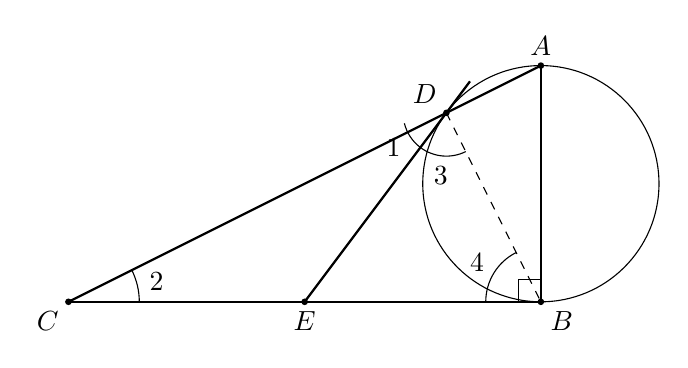
\begin{tikzpicture}[scale=1.0]
  \coordinate (B) at (0,0);
  \coordinate (A) at (0,3);
  \coordinate (C) at (-6,0);
  \coordinate (O) at (0,1.5);
  \coordinate (D) at (-1.2,2.4);
  \coordinate (E) at (-3,0);
  \coordinate (T) at (-0.9,2.8);
  \draw (O) circle (1.5);
  \draw[thick] (C)--(A);
  \draw[thick] (A)--(B);
  \draw[thick] (C)--(B);
  \draw[thick] (E)--(T);
  \draw[dashed] (D)--(B);
  \fill (A) circle (1.2pt) node[above] {$A$};
  \fill (B) circle (1.2pt) node[below right] {$B$};
  \fill (C) circle (1.2pt) node[below left] {$C$};
  \fill (D) circle (1.2pt) node[above left] {$D$};
  \fill (E) circle (1.2pt) node[below] {$E$};
  % ∠2（C 处，CB 与 CA 之间）
  \draw ([shift={(0:0.9)}]C) arc (0:26.57:0.9);
  \node at (-4.88,0.26) {$2$};
  % ∠1（D 处，DC 与 DE 之间）
  \draw ([shift={(194.04:0.55)}]D) arc (194.04:233.13:0.55);
  \node at (-1.87,1.96) {$1$};
  % ∠3（D 处，DE 与 DB 之间）
  \draw ([shift={(233.13:0.55)}]D) arc (233.13:296.57:0.55);
  \node at (-1.27,1.60) {$3$};
  % ∠4（B 处，BD 与 BC 之间）
  \draw ([shift={(116.57:0.7)}]B) arc (116.57:180:0.7);
  \node at (-0.81,0.50) {$4$};
  % B 处直角记号（∠ABC=90°）
  \draw (0,0.28)--(-0.28,0.28)--(-0.28,0);
\end{tikzpicture}
\end{center}
\nopagebreak[4]
\Needspace{4\baselineskip}
\textbf{解析}
\nopagebreak[4]
\begin{center}% 1977 年贵州卷第三题：直角三角形 ABC（∠ABC=90°），以直角边 AB 为直径作园，
% 园与斜边 AC 交于 D，过 D 的切线交 BC 于 E（切线向 D 上方延长），
% 虚线为辅助线 BD；角标注 ∠1（CDE）、∠2（DCE）、∠3（EDB）、∠4（DBE），
% B 处另画直角记号（按源卷第 3 页布局，几何关系自洽：ED=EB=3）
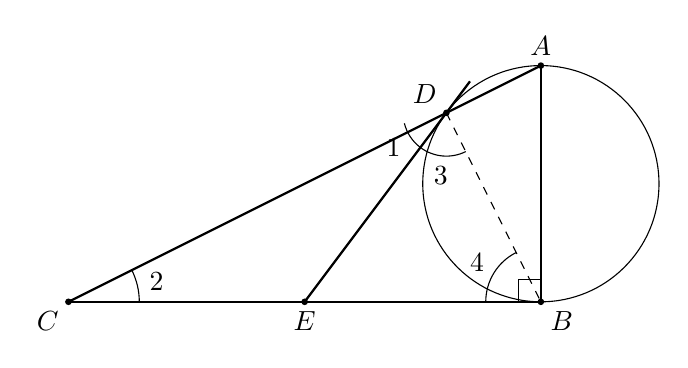
\begin{tikzpicture}[scale=1.0]
  \coordinate (B) at (0,0);
  \coordinate (A) at (0,3);
  \coordinate (C) at (-6,0);
  \coordinate (O) at (0,1.5);
  \coordinate (D) at (-1.2,2.4);
  \coordinate (E) at (-3,0);
  \coordinate (T) at (-0.9,2.8);
  \draw (O) circle (1.5);
  \draw[thick] (C)--(A);
  \draw[thick] (A)--(B);
  \draw[thick] (C)--(B);
  \draw[thick] (E)--(T);
  \draw[dashed] (D)--(B);
  \fill (A) circle (1.2pt) node[above] {$A$};
  \fill (B) circle (1.2pt) node[below right] {$B$};
  \fill (C) circle (1.2pt) node[below left] {$C$};
  \fill (D) circle (1.2pt) node[above left] {$D$};
  \fill (E) circle (1.2pt) node[below] {$E$};
  % ∠2（C 处，CB 与 CA 之间）
  \draw ([shift={(0:0.9)}]C) arc (0:26.57:0.9);
  \node at (-4.88,0.26) {$2$};
  % ∠1（D 处，DC 与 DE 之间）
  \draw ([shift={(194.04:0.55)}]D) arc (194.04:233.13:0.55);
  \node at (-1.87,1.96) {$1$};
  % ∠3（D 处，DE 与 DB 之间）
  \draw ([shift={(233.13:0.55)}]D) arc (233.13:296.57:0.55);
  \node at (-1.27,1.60) {$3$};
  % ∠4（B 处，BD 与 BC 之间）
  \draw ([shift={(116.57:0.7)}]B) arc (116.57:180:0.7);
  \node at (-0.81,0.50) {$4$};
  % B 处直角记号（∠ABC=90°）
  \draw (0,0.28)--(-0.28,0.28)--(-0.28,0);
\end{tikzpicture}
\end{center}
\nopagebreak[4]
\Needspace{5\baselineskip}
如图，连接 $BD$（图中虚线）。因为 $AB$ 为直径，所以 $\angle ADB=90^{\circ}$（直径所对的圆周角）。因为 $\angle ABC=90^{\circ}$ 且 $E$ 在 $BC$ 上，$EB\perp AB$，故 $EB$ 是园在点 $B$ 处的切线；$ED$ 已是切线，于是 $ED$ 与 $EB$ 是从园外一点 $E$ 引出的两条切线（切线长定理），

\nopagebreak[4]
\[
ED=EB\qquad\text{……（1）}
\]

从而 $\angle3=\angle4$（等腰三角形 $EDB$ 的底角）。

\Needspace{5\baselineskip}
又 $C$、$D$、$A$ 共线，故 $\angle CDB=180^{\circ}-\angle ADB=90^{\circ}$，即

\nopagebreak[4]
\[
\angle1+\angle3=90^{\circ}.
\]

\Needspace{5\baselineskip}
$\angle2$（即 $\angle ACB$）与 $\angle ABD$ 分别是直角三角形 $ABC$、$ABD$ 中同一个锐角 $\angle A$ 的余角，故 $\angle2=\angle ABD$；而 $\angle ABD+\angle4=\angle ABC=90^{\circ}$，因此

\nopagebreak[4]
\[
\angle2+\angle4=90^{\circ}.
\]

\Needspace{5\baselineskip}
由 $\angle3=\angle4$ 得 $\angle1=\angle2$；在 $\triangle CDE$ 中，等角对等边，

\nopagebreak[4]
\[
CE=ED\qquad\text{……（2）}
\]

\Needspace{5\baselineskip}
由（1）和（2）即得

\nopagebreak[4]
\[
EB=CE.
\]

\gkanswer{答案：见解析版}

\end{answer}
\begin{answer}
\gksolhead{4}{}

\textbf{题目}：

求到点 $A(1,2)$ 和点 $B(4,1)$ 等距离的点的轨迹的方程。

\Needspace{4\baselineskip}
\textbf{解析}

\Needspace{5\baselineskip}
设 $P(x,y)$ 是到 $A$、$B$ 等距离的任意一点，则 $|PA|=|PB|$。由两点间距离公式，

\nopagebreak[4]
\[
\sqrt{(x-1)^{2}+(y-2)^{2}}=\sqrt{(x-4)^{2}+(y-1)^{2}}.
\]

\Needspace{5\baselineskip}
两边平方，展开：

\nopagebreak[4]
\[
x^{2}-2x+1+y^{2}-4y+4=x^{2}-8x+16+y^{2}-2y+1,
\]

\Needspace{5\baselineskip}
整理得

\nopagebreak[4]
\[
6x-2y-12=0,
\]

\Needspace{5\baselineskip}
即所求轨迹（线段 $AB$ 的垂直平分线）方程为

\nopagebreak[4]
\[
3x-y-6=0\qquad(\text{\text{即} }y=3x-6).
\]

\gkanswer{答案：$3x-y-6=0$（即 $y=3x-6$）。}

\end{answer}
\begin{answer}
\gksolhead{5}{}

\textbf{题目}：

用长 $8$ 米的木料，做一矩形的窗框，问长和宽如何选择，才能使窗子透过的光线最多？

\Needspace{4\baselineskip}
\textbf{解析}

\Needspace{5\baselineskip}
设窗子的宽为 $x$ 米，则长为 $(4-x)$ 米，窗子面积

\nopagebreak[4]
\[
S=x(4-x)=-\left(x-2\right)^{2}+4\leqslant4.
\]

当 $x=2$ 时 $S$ 取最大值 $4$，此时长为 $4-2=2$ 米。故窗子的长、宽相等且均为 $2$ 米（边长 $2$ 米的正方形）时，透过的光线最多。

\gkanswer{答案：当长、宽相等且均为 $2$ 米（边长 $2$ 米的正方形）时，窗子透过的光线最多。}

\end{answer}
\begin{answer}
\gksolhead{6}{}

\textbf{题目}：

求 $\operatorname{Lim}_{n\to\infty}a\sin\alpha\left(1+\cos\alpha+\cos^{2}\alpha+\cdots+\cos^{n}\alpha\right)=?$（其中 $a$ 为任意实常数，$0<\alpha<\dfrac{\pi}{2}$）

\Needspace{4\baselineskip}
\textbf{解析}

\Needspace{5\baselineskip}
数列 $1,\ \cos\alpha,\ \cos^{2}\alpha,\ \cdots$ 的公比 $q=\cos\alpha$。由 $0<\alpha<\dfrac{\pi}{2}$ 得 $0<q<1$，是无穷递缩等比数列，其和为

\nopagebreak[4]
\[
\operatorname{Lim}_{n\to\infty}\left(1+\cos\alpha+\cdots+\cos^{n}\alpha\right)=\frac{1}{1-\cos\alpha}.
\]

\Needspace{5\baselineskip}
于是

\nopagebreak[4]
\[
\operatorname{Lim}_{n\to\infty}a\sin\alpha\left(1+\cos\alpha+\cos^{2}\alpha+\cdots+\cos^{n}\alpha\right)
=\frac{a\sin\alpha}{1-\cos\alpha}.
\]

\Needspace{5\baselineskip}
由半角公式 $\sin\alpha=2\sin\dfrac{\alpha}{2}\cos\dfrac{\alpha}{2}$，$1-\cos\alpha=2\sin^{2}\dfrac{\alpha}{2}$，

\nopagebreak[4]
\[
\frac{a\sin\alpha}{1-\cos\alpha}
=\frac{2a\sin\frac{\alpha}{2}\cos\frac{\alpha}{2}}{2\sin^{2}\frac{\alpha}{2}}
=a\cot\frac{\alpha}{2}.
\]

\begin{gktip}
\textbf{源注}：源解答中「$\cos^n x$」「$a\,\operatorname{ctg} x/2$」两处的「$x$」均为「$\alpha$」的排印误植；本文按 $\alpha$ 计算。
\end{gktip}

\gkanswer{答案：$a\cot\dfrac{\alpha}{2}$。}

\end{answer}
\begin{answer}
\gksolhead{7}{}

\textbf{题目}：

\Needspace{5\baselineskip}
已知方程 $x^{2}+px+q=0$ 的两个根为 $\operatorname{tg}\alpha$ 与 $\operatorname{tg}\beta$，求

\nopagebreak[4]
\[
\sin^{2}(\alpha+\beta)+p\sin(\alpha+\beta)\cos(\alpha+\beta)+q\cos^{2}(\alpha+\beta)
\]

的值，（其中 P、q 为任意实常数）。

\begin{gktip}
\textbf{源注}：括注中的大写「P」系源卷排印（题中系数实为 $p$），照录。
\end{gktip}

\Needspace{4\baselineskip}
\textbf{解析}

\Needspace{5\baselineskip}
由一元二次方程根与系数的关系，

\nopagebreak[4]
\[
\operatorname{tg}\alpha+\operatorname{tg}\beta=-p,
\qquad
\operatorname{tg}\alpha\cdot\operatorname{tg}\beta=q.
\]

\Needspace{5\baselineskip}
当 $q\neq1$ 时，$\operatorname{tg}(\alpha+\beta)=\dfrac{\operatorname{tg}\alpha+\operatorname{tg}\beta}{1-\operatorname{tg}\alpha\operatorname{tg}\beta}=\dfrac{-p}{1-q}$，于是

\nopagebreak[4]
\[
\begin{aligned}
&\sin^{2}(\alpha+\beta)+p\sin(\alpha+\beta)\cos(\alpha+\beta)+q\cos^{2}(\alpha+\beta)\\
&=\cos^{2}(\alpha+\beta)\left[\operatorname{tg}^{2}(\alpha+\beta)+p\operatorname{tg}(\alpha+\beta)+q\right]\\
&=\frac{\operatorname{tg}^{2}(\alpha+\beta)+p\operatorname{tg}(\alpha+\beta)+q}{1+\operatorname{tg}^{2}(\alpha+\beta)}\\
&=\frac{\dfrac{p^{2}}{(1-q)^{2}}-\dfrac{p^{2}}{1-q}+q}{1+\dfrac{p^{2}}{(1-q)^{2}}}.
\end{aligned}
\]

\Needspace{5\baselineskip}
分子通分：

\nopagebreak[4]
\[
\frac{p^{2}-p^{2}(1-q)+q(1-q)^{2}}{(1-q)^{2}}
=\frac{q\left[p^{2}+(1-q)^{2}\right]}{(1-q)^{2}},
\]

\Needspace{5\baselineskip}
分母通分：

\nopagebreak[4]
\[
\frac{p^{2}+(1-q)^{2}}{(1-q)^{2}}.
\]

\Needspace{5\baselineskip}
相除即得

\nopagebreak[4]
\[
q.
\]

当 $q=1$ 时，$1-\operatorname{tg}\alpha\operatorname{tg}\beta=0$，故 $\alpha+\beta=\dfrac{\pi}{2}+k\pi$（$k$ 为整数），$\cos(\alpha+\beta)=0$、$\sin(\alpha+\beta)=\pm1$，原式只剩 $\sin^{2}(\alpha+\beta)=1$。

\gkanswer{答案：$q\neq1$ 时原式等于 $q$；$q=1$ 时原式等于 $1$。}

\end{answer}
\begin{answer}
\gksolhead{8}{}

\textbf{题目}：

设有直线（L）与曲线（c）：直线（L）：$y=ax-1$；曲线（c）：$r\sin\theta=\sin2\theta$。问（L）与（c）在什么条件下相交、相切、不相交。

\textbf{参考题 1．} 设某平板上任意一点的电势，在 $\rho\geqslant1$ 时，由 $E=\operatorname{Ln}\rho$ 给出，这里 $\rho$ 是以原点为起点的矢径。试求在点 $\rho=5$，$C-\arcsin 0.8$ 处，沿此点至 $\rho=10$，$\theta=\dfrac{\pi}{2}$ 的方向 $E$ 的变化率。

\begin{gktip}
\textbf{源注}：源卷题面印作「C—arcsin0.8」；同页解答及答句均作「$\theta=\arcsin 0.8$」（对应直角坐标点 $(3,4)$），「C—」系「$\theta=$」的排印误植，题面照录原样并在此说明。
原源 PDF 第 5 页附有直角坐标系、点 $(3,4)$、$(0,10)$ 与方向向量 $\vec{l}$ 的示意图；LaTeX 版按源图重绘。
\end{gktip}
\nopagebreak[4]
\begin{center}% 1977 年贵州卷参考题一：直角坐标系、刻度、单位向量 i 与 j、
% 点 (3,4) 与 (0,10)、虚线向两轴投影、方向向量 l 从 (3,4) 指向 (0,10)
% （按源卷第 5 页布局）
\begin{tikzpicture}[>=stealth,scale=0.85]
  \draw[->] (-0.7,0)--(7,0) node[below] {$x$};
  \draw[->] (0,-0.7)--(0,11) node[left] {$y$};
  \foreach \t in {2,4,6} \draw (\t,0.12)--(\t,-0.12) node[below] {$\t$};
  \foreach \t in {2,4,6,8,10} \draw (0.12,\t)--(-0.12,\t) node[left] {$\t$};
  % 单位向量
  \draw[->,thick] (0,0)--(0.9,0);
  \node at (0.5,-0.55) {$\vec{i}$};
  \draw[->,thick] (0,0)--(0,0.9);
  \node at (-0.55,0.5) {$\vec{j}$};
  % 虚线投影
  \draw[dashed] (3,0)--(3,4)--(0,4);
  % 方向向量
  \draw[->,very thick] (3,4)--(0,10);
  \node at (1.95,6.9) {$\vec{l}$};
  \fill (3,4) circle (2pt) node[right] {$(3,4)$};
  \fill (0,10) circle (2pt) node[above right] {$(0,10)$};
  \node at (0,0) [below left] {$0$};
\end{tikzpicture}
\end{center}
\nopagebreak[4]
\Needspace{5\baselineskip}
\textbf{参考题 2．} 证明

\nopagebreak[4]
\[
S_{1}=1,\quad S_{2}=1+\frac{1}{2^{2}},\quad S_{3}=1+\frac{1}{2^{2}}+\frac{1}{3^{2}},\ \cdots,\quad S_{n}=1+\frac{1}{2^{2}}+\frac{1}{3^{2}}+\cdots+\frac{1}{n^{2}},\ \cdots
\]

是收敛叙列。

\begin{gktip}
\textbf{源注}：源卷首项印作「S,=1」，系下标 1 误印为逗号，本文按 $S_{1}=1$ 转录；「叙列」为源卷排印用字，照录。
\end{gktip}

\Needspace{4\baselineskip}
\textbf{解析}

\Needspace{5\baselineskip}
由 $\sin2\theta=2\sin\theta\cos\theta$ 以及 $x=r\cos\theta$、$y=r\sin\theta$，$\sin2\theta=2\cdot\dfrac{y}{r}\cdot\dfrac{x}{r}=\dfrac{2xy}{x^{2}+y^{2}}$，方程 $r\sin\theta=\sin2\theta$ 化为

\nopagebreak[4]
\[
y=\frac{2xy}{x^{2}+y^{2}}.
\]

\Needspace{5\baselineskip}
$y\neq0$ 时约去 $y$ 得 $x^{2}+y^{2}=2x$；$y=0$ 时 $\sin\theta=0$，原方程恒成立，极点 $(0,0)$ 在曲线上，且也满足 $x^{2}+y^{2}=2x$。故曲线（c）为整圆

\nopagebreak[4]
\[
\left(x-1\right)^{2}+y^{2}=1.
\]

\Needspace{5\baselineskip}
解方程组

\nopagebreak[4]
\[
\begin{cases}
y=ax-1,\\
(x-1)^{2}+y^{2}=1,
\end{cases}
\]

\Needspace{5\baselineskip}
将 $y=ax-1$ 代入圆方程，整理得

\nopagebreak[4]
\[
(1+a^{2})x^{2}-2(a+1)x+1=0.
\]

\Needspace{5\baselineskip}
其判别式

\nopagebreak[4]
\[
\Delta=4(a+1)^{2}-4(1+a^{2})=8a.
\]

$\Delta>0$（$a>0$）时方程组有两组不同实解，直线与圆有两个交点，即相交；$\Delta=0$（$a=0$）时只有一组解，即相切；$\Delta<0$（$a<0$）时无实解，即不相交。故 $a>0$ 时相交，$a=0$ 时相切，$a<0$ 时不相交。

\begin{gktip}
\textbf{源注}：源解答把判别式两处印作「(4a+1)²$-$4(1+a²)」「4(a+1)²$-$(1+a²)」，均为「4(a+1)²$-$4(1+a²)」的排印误植（所得结果 $8a$ 正确）。
\end{gktip}

\textbf{参考题 1}
\nopagebreak[4]
\begin{center}% 1977 年贵州卷参考题一：直角坐标系、刻度、单位向量 i 与 j、
% 点 (3,4) 与 (0,10)、虚线向两轴投影、方向向量 l 从 (3,4) 指向 (0,10)
% （按源卷第 5 页布局）
\begin{tikzpicture}[>=stealth,scale=0.85]
  \draw[->] (-0.7,0)--(7,0) node[below] {$x$};
  \draw[->] (0,-0.7)--(0,11) node[left] {$y$};
  \foreach \t in {2,4,6} \draw (\t,0.12)--(\t,-0.12) node[below] {$\t$};
  \foreach \t in {2,4,6,8,10} \draw (0.12,\t)--(-0.12,\t) node[left] {$\t$};
  % 单位向量
  \draw[->,thick] (0,0)--(0.9,0);
  \node at (0.5,-0.55) {$\vec{i}$};
  \draw[->,thick] (0,0)--(0,0.9);
  \node at (-0.55,0.5) {$\vec{j}$};
  % 虚线投影
  \draw[dashed] (3,0)--(3,4)--(0,4);
  % 方向向量
  \draw[->,very thick] (3,4)--(0,10);
  \node at (1.95,6.9) {$\vec{l}$};
  \fill (3,4) circle (2pt) node[right] {$(3,4)$};
  \fill (0,10) circle (2pt) node[above right] {$(0,10)$};
  \node at (0,0) [below left] {$0$};
\end{tikzpicture}
\end{center}
\nopagebreak[4]
\Needspace{5\baselineskip}
由 $\rho=\sqrt{x^{2}+y^{2}}$，$E=\operatorname{Ln}\rho=\operatorname{Ln}\sqrt{x^{2}+y^{2}}$，

\nopagebreak[4]
\[
\frac{\partial E}{\partial x}=\frac{x}{x^{2}+y^{2}},
\qquad
\frac{\partial E}{\partial y}=\frac{y}{x^{2}+y^{2}}.
\]

\Needspace{5\baselineskip}
点 $\rho=5$、$\theta=\arcsin 0.8$（$\sin\theta=0.8$、$\cos\theta=0.6$，第一象限）即点 $(3,4)$；终点 $\rho=10$、$\theta=\dfrac{\pi}{2}$ 即点 $(0,10)$。方向向量

\nopagebreak[4]
\[
\vec{l}=(0-3)\vec{i}+(10-4)\vec{j}=-3\vec{i}+6\vec{j},
\qquad
\left|\vec{l}\right|=3\sqrt{5},
\]

\Needspace{5\baselineskip}
方向余弦

\nopagebreak[4]
\[
\cos\alpha=\frac{-3}{3\sqrt{5}}=-\frac{1}{\sqrt{5}},
\qquad
\cos\beta=\frac{6}{3\sqrt{5}}=\frac{2}{\sqrt{5}}.
\]

\Needspace{5\baselineskip}
于是

\nopagebreak[4]
\[
\frac{\partial E}{\partial\vec{l}}
=-\frac{1}{\sqrt{5}}\cdot\frac{x}{x^{2}+y^{2}}
+\frac{2}{\sqrt{5}}\cdot\frac{y}{x^{2}+y^{2}}.
\]

\Needspace{5\baselineskip}
在点 $(3,4)$ 处（$x^{2}+y^{2}=25$）：

\nopagebreak[4]
\[
\frac{\partial E}{\partial\vec{l}}\bigg|_{(3,4)}
=-\frac{1}{\sqrt{5}}\cdot\frac{3}{25}
+\frac{2}{\sqrt{5}}\cdot\frac{4}{25}
=\frac{5}{25\sqrt{5}}
=\frac{\sqrt{5}}{25}.
\]

即 $E$ 沿该方向的变化率为 $\dfrac{\sqrt{5}}{25}$。

\textbf{参考题 2}

因为 $S_{n}-S_{n-1}=\dfrac{1}{n^{2}}>0$，所以 $\{S_{n}\}$ 单调递增。

\Needspace{5\baselineskip}
又

\nopagebreak[4]
\[
S_{n}=1+\frac{1}{2^{2}}+\frac{1}{3^{2}}+\cdots+\frac{1}{n^{2}}
<1+\frac{1}{1\cdot2}+\frac{1}{2\cdot3}+\cdots+\frac{1}{(n-1)n}
=1+\left(1-\frac{1}{n}\right)=2-\frac{1}{n}<2,
\]

这里 $k\geqslant2$ 时 $\dfrac{1}{k^{2}}<\dfrac{1}{(k-1)k}$，即 $\{S_{n}\}$ 有上界。单调递增而有上界的数列必收敛，故 $\{S_{n}\}$ 收敛。

\gkanswer{答案：$a>0$ 时（L）与（c）相交；$a=0$ 时相切；$a<0$ 时不相交。}

\end{answer}